\begin{wrapfigure}{r}{0.4\textwidth}
    \vspace{-0.4cm}
    \centering
    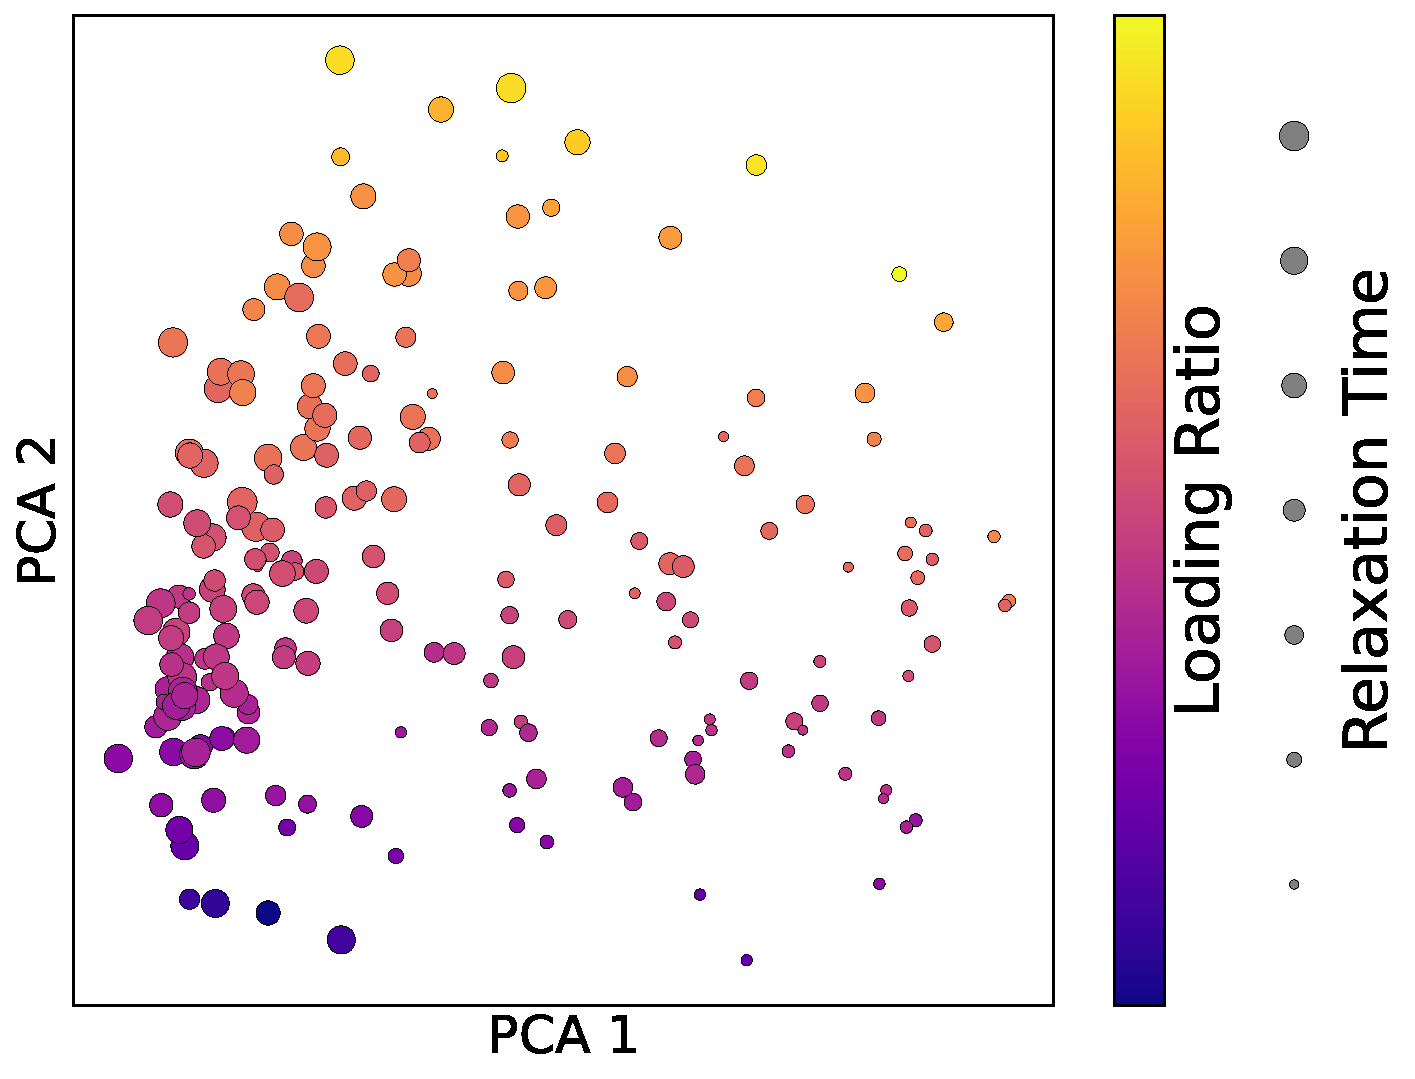
\includegraphics[width=\linewidth]{figures/latent_space_vis/pca_peach_trampoline_bivariate.pdf}
\caption{
    Visualization of the first and second PCA component of the latent space on the \texttt{Trampoline} dataset.
    Each point represents one simulation test task.
    Color corresponds to ratio of mass to product of Young's modulus and sheet thickness, i.e., loading ratio, which governs the degree of sheet deformation.
    Size corresponds to relaxation time.
    }
    \vspace{-0.4cm}
    \label{fig:latent_space_vis_main}
\end{wrapfigure}
